V telekomunikacích se používají filtry v rozsahu kmitočtů desítek až stovek megahertz, v bezdrátové komunikaci až v řádu gigahertz. Běžné RC filtry by neměly být užívány ve frekvenčním rozsahu nad 5--10 $\%$ $\omega _c$ - tedy v tomto rozsahu používaném v telekomunikačních technologiích nemají předvídatelné průběhy. Krom toho ve spínačích CMOS, kde rezistory běžně nejsou dostupné, jsou potřeba zesilovače s velkou šířkou pásma a zároveň vysokým zesílením. Dodržení těchto požadavků je náročné a drahé. Dalším extrémem pro analogové integrované filtry jsou telefonní linky, kde jsou kmitočtové rozsahy sice nízké, ale je požadována nízká cena a vysoká přesnost.\\
\\
Pro nízké frekvence se ke splnění těchto požadavků používají obvody se spínanými kapacitory (SC). Přepínaný kapacitor se chová jako rezistor, tudíž časová konstanta RC je definována poměrem kapacitorů a hodinovou (CLK) frekvencí, se kterou jsou přepínány. Pro vysokofrekvenční aplikace (až v řádu gigahertz) se používají MOSFET-C filtry.\\
\\
Další z možných prvků, které jsou dostupné jak pro nízkofrekvenční aplikace, tak pro kmitočtový rozsah stovek megahertz, jsou transkonduktanční zesilovače. Jejich kmitočtové vlastnosti umožňují využití při konstrukci ARC (\textit{Active RC}) filtrů v pracovním kmitočtovém pásmu do cca 10 MHz a se speciálně konstruovanými OTA až do 100 MHz.\\
\\
Transkonduktanční zesilovače (označují se též jako OTA (\textit{Operational Transconductance Amplifiers}) jsou napětím řízené zesilovače s proudovým výstupem - zdroje proudu
\begin{equation}
i_{out} = g_m(u_+ - u_-),
\end{equation}
kde $u_+$ a $u_-$ jsou napětí invertujícího a neinvertujícího vstupu.  Transkonduktance je řízena externím proudem $I_{ABC}$ (\textit{Bias Current}). Ideální OTA má kmitočtově nezávislou transkonduktanci $g_m$ (na rozdíl od reálného, který je kmitočtově závislý).
\begin{figure}[h]
\centering
\includegraphics[scale=0.7]{image7.png}
\caption[OTA - schematické značky]{OTA - schematické značky \cite{4}}
\end{figure}
\begin{figure}[h]
\centering
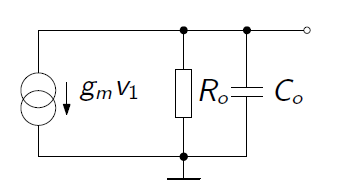
\includegraphics[scale=0.6]{gmrc.png}
\caption[Linearizovaný model reálného OTA]{Linearizovaný model reálného OTA \cite{5}}
\end{figure}
\noindent Připojením zátěže $R_z$ na výstup bylo získáno napětí naprázdno
\begin{equation}\label{s:vzt}
u_{out} = R_zg_m(u_+ - u_-) = G_0(u_+ - u_-),
\end{equation}
kde $G_0$ je zesílení. Ze vztahu \ref{s:vzt} plyne, že zesílení je konečné a mezi vstupy je nenulové napětí. \\
\noindent Po připojení kondenzátoru jako zátěže byl získán bezeztrátový integrátor s přenosem
\begin{equation}
H(s) = \frac{v_2}{v_1} = \frac{g_m}{pC}
\end{equation}
\noindent a napětím na výstupu
\begin{equation}
v_0(t) = \frac{1}{C}\int i(t)dt = \frac{1}{C}\int g_mv_1(t)dt.
\end{equation}
\begin{figure}[h]
\centering
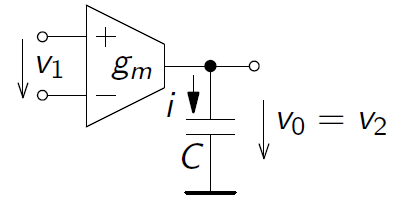
\includegraphics[scale=0.5]{otaintegrator.png}
\caption[OTA-C]{OTA-C \cite{5} \label{s:GM-C}}
\end{figure}
\noindent Toto zapojení integrátoru s uzemněným kondenzátorem se označuje jako OTA-C.\\
\\
Ztrátový integrátor lze utvořit sériovým zapojením dalšího OTA jako odporu se zápornou zpětnou vazbou. Rozdíl mezi ideálním a ztrátovým integrátorem lze pozorovat i v modulové charakteristice - pro ztrátový je konstantní a pak teprve lineárně klesá se sklonem -20 dB/dek.\\
Po doplnění ztrátové vodivosti, kterou zde simuluje druhý zesilovač, paralelně k integrační kapacitě, byl obdržen vztah pro výstupní napětí
\begin{equation}
v_0(t) = \frac{g_{m1}}{sC + g_{m2}}(v_1^+ - v_{1}^-).
\end{equation}
\begin{figure}[h]
\centering
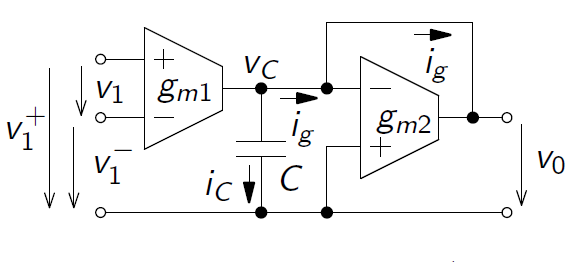
\includegraphics[scale=0.5]{damp.png}
\caption[Ztrátový OTA-C]{Ztrátový OTA-C \cite{5}}
\end{figure}
\subsection{Proudový konvejor druhé generace s OTA}
Jeden z nejzákladnějších bloků v oblasti analogov obvodů v proudovém módu je proudový konvejor (\textit{current conveyor (CC)}). Princip CC první generace byl popsán v roce 1968 (K. C. Smith, A. S. Sedra \cite{6}). \textit{CCI} byl následně nahrazen univerzálnější druhou generací v roce 1970 (\textit{CCII})\cite{7}. Obvody s CC se používaly především v zapojeních s bipolárními tranzistory kvůli jejich vysoké transkonduktanci (v porovnání s CMOS). Jsou to operační zesilovače s proudovou zpětnou vazbou (např. MAX477, MAX4112). Proudové konvejory (\textit{Current conveyors}) jsou používány ve vysokofrekvenčních obvodech, kde je problematické použití běžných operačních zesilovačů, protože jsou limitovány násobkem šířky pásma a zesílení (\textit{gain-bandwidth product}). Je to struktura s třemi vstupy.
\begin{figure}[h]
\centering
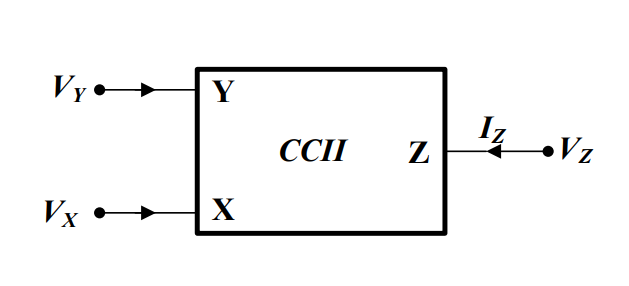
\includegraphics[scale=0.4]{ccii.png}
\caption[CCII symbol]{CCII symbol \cite{8}}
\end{figure}
\noindent Proudovým konvejorem lze také jednoduše realizovat integrátor. Pro výstupní napětí $u_0$ obvodu a z něj odvozenou přenosovou funkci platí
\begin{align}
u_0(t) &= \frac{1}{C}\int i_c(t)dt = \frac{1}{RC}\int u_{in}(t)dt \\
H(p) &= \frac{U_2}{U_1} = \frac{1}{pCR}.
\end{align}
\noindent Konvejorový integrátor pracuje jako invertující nebo neinvertující.
\begin{figure}[h]
\centering
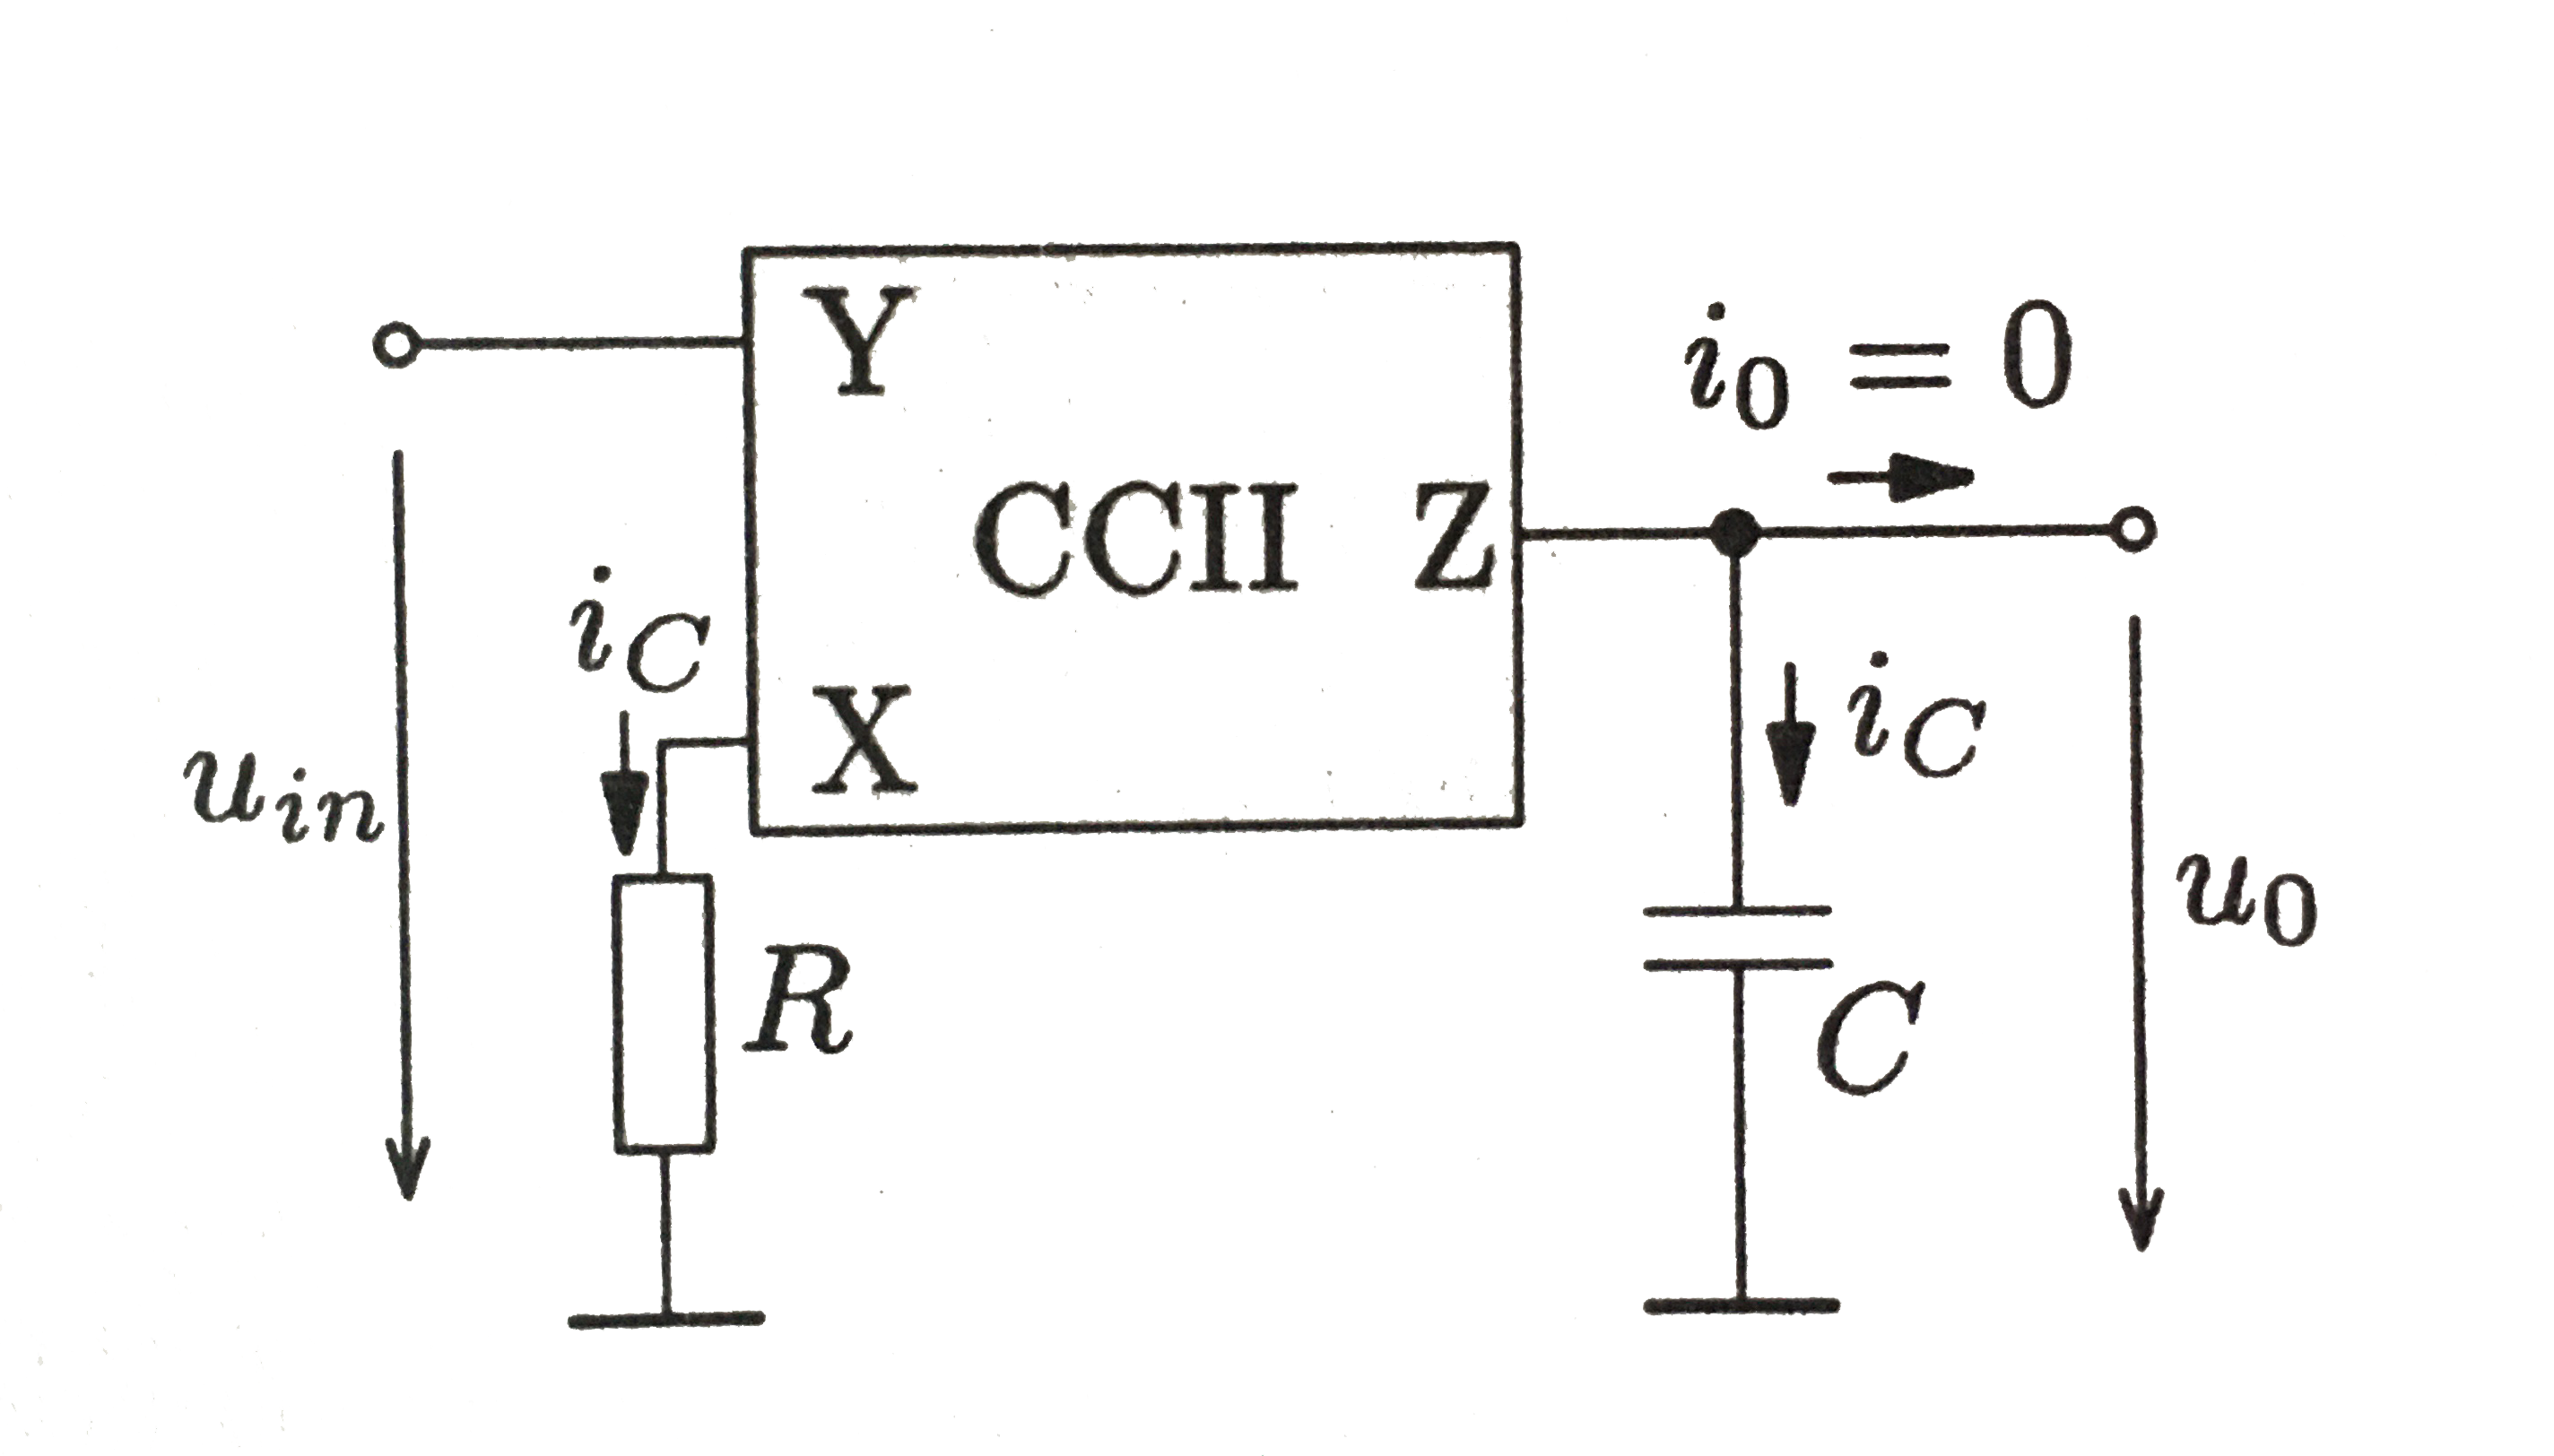
\includegraphics[scale=0.075]{ccii_int1.png}
\caption[Integrátor s CCII a OTA]{Integrátor s CCII a OTA \cite{3}}
\end{figure}
\noindent Vstupní impedance na vstupu Y je nekonečná (tedy proud tekoucí skrz Y je nulový) a impedance na vstupu X je nulová ($R_Y = \infty, I_Y = 0, R_X = 0$). Napětí na vstupu X je ekvivalentní k napětí na vstupu Y ($V_X = V_Y$). Proud procházející vstupem X je ekvivalentní k proudu vstupem Z ($I_Z = I_X$). Výstupní impedance vstupu Z je nekonečná ($R_Z = \infty$).
Charakteristika ideálního \textit{CC} je reprezentována maticí
\begin{equation}
\begin{bmatrix}
I_Y \\ V_X \\ I_Z
\end{bmatrix}
=
\begin{bmatrix}
0 & 0 & 0 \\
1 & 0 & 0 \\
0 & \pm 1 & 0 
\end{bmatrix}
\begin{bmatrix}
V_Y \\
I_X \\
V_Z
\end{bmatrix}.
\end{equation}
\begin{figure}[h]
\centering
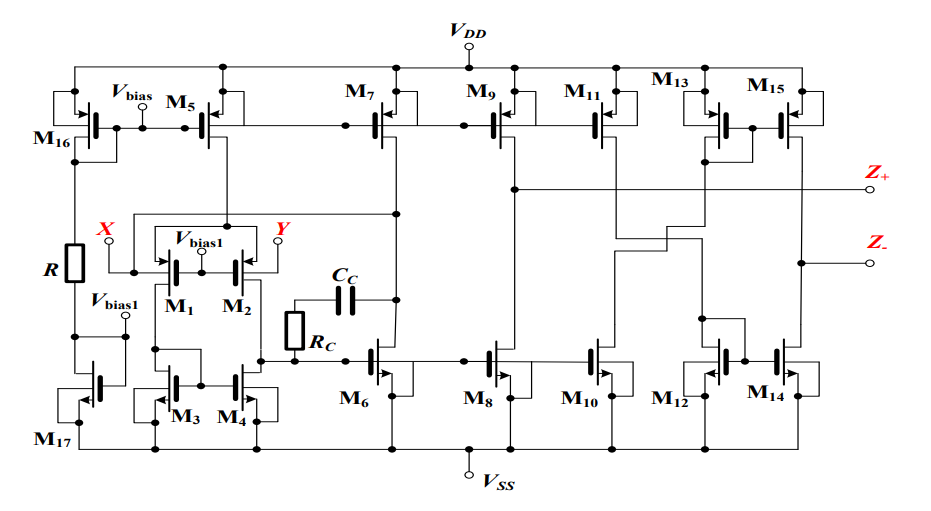
\includegraphics[scale=0.45]{cciiota.png}
\caption[CCII s $\pm$ výstupem založený na OTA]{CCII s $\pm$ výstupem založený na OTA \cite{8}}
\end{figure}
\newline
V analogových IC je preferováno diferenční zpracování signálů, protože redukuje zkreslení a šum (diferenční stupeň vyruší kladné a záporné výchylky napětí/proudu např. na zdroji a také vyruší nelinearity způsobené zesilovačem).\\
Využitím zapojení na obrázku \ref{s:OTA} a principů \textit{CCII} lze získat modifikace klasického transkonduktančního zesilovače (s rozdílovým stupněm na vstupu a jedním výstupem). Obdržené atypické struktury obsahují jeden vstup a jeden výstup a také dva rozdílové stupně (na vstupu i výstupu). Provodení diferenčního stupně na výstupu je znázorněno na obrázku \ref{s:CMOS}. Takovéto zapojení funguje jako dobrý sledovač napětí, ale zato má menší šířku pásma. Také má menší transkonduktanci, protože každou polovinou diferenčního obvodu teče jen polovina vstupního proudu (\textit{bias current}). Problémem je také relativně nízké stejnosměrné zesílení, proto se v praxi se zapojením s OTA nepoužívá. \\
\begin{figure}[h]
\centering
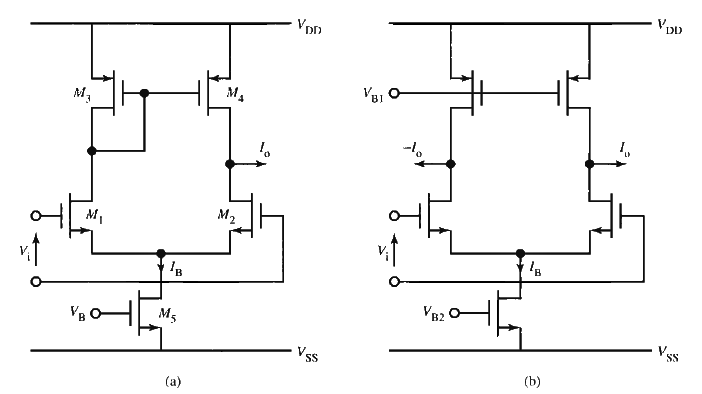
\includegraphics[scale=0.5]{diff.png}
\caption[Základní CMOS transkonduktance a) jeden výstup b) diferenční výstup]{Základní CMOS transkonduktance a) jeden výstup b) diferenční výstup \cite{12} \label{s:CMOS}}
\end{figure}
\begin{figure}[h]
\centering
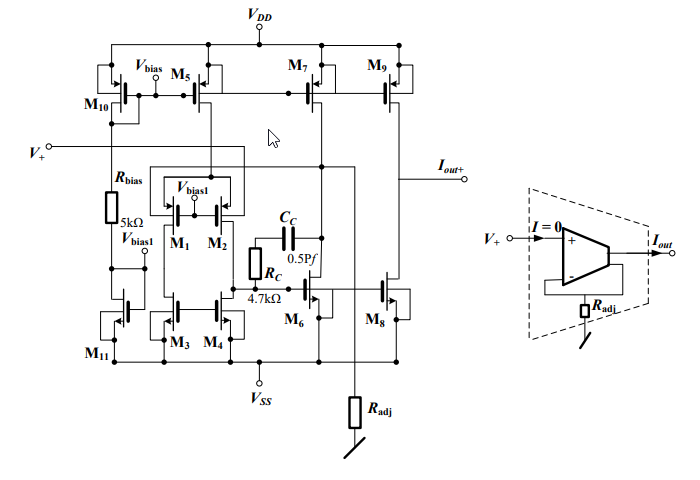
\includegraphics[scale=0.6]{siso.png}
\caption[Single input single output OTA (SISO) založený na CCII]{Single input single output OTA (SISO) založený na CCII \cite{8}}
\end{figure}
\begin{figure}[h]
\centering
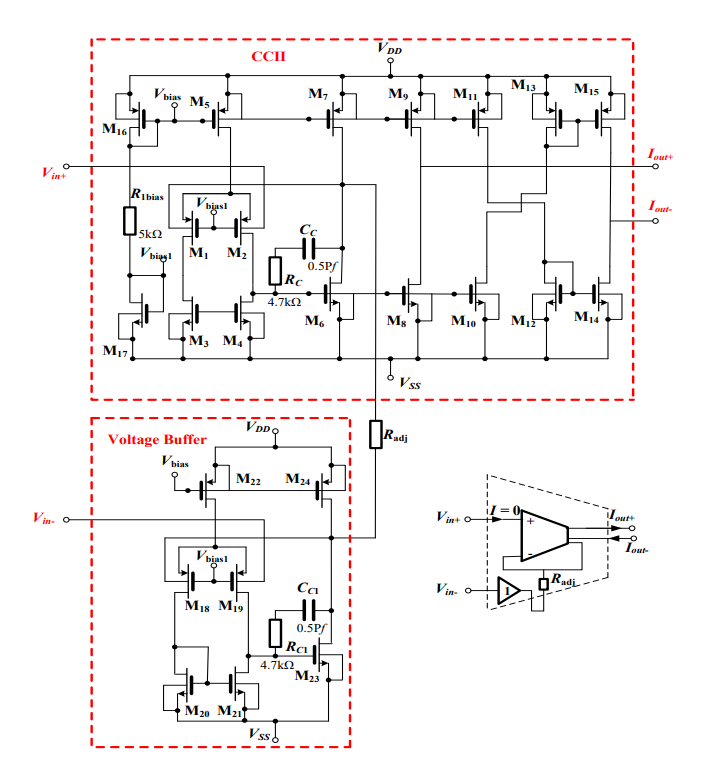
\includegraphics[scale=0.5]{dido.png}
\caption[\textit{Fully differential} OTA (DIDO) založený na CCII a napěťovém bufferu]{\textit{Fully differential} OTA (DIDO) založený na CCII a napěťovém bufferu \cite{8}}
\end{figure}
\newpage
\subsection{IC s OTA}
OTA bývá nejčastěji implementován v unipolární monolitické technologii (CMOS) a v případě, že se jedná o reálný prvek, má převážně kapacitní charakter (vstupní impedance se stává kapacitou). Integrované obvody se vyrábí buď s jedním nebo dvěma zesilovači v pouzdře. Varianty s jedním operačním zesilovačem jsou např. OPA615, OPA860 a novější OPA861. Všechny součástky s jedním OTA mají velkou šířku pásma (v řádech stovek MHz), cenově vychází na 75--280 Kč. IC s dvěma zesilovači v pouzdře mají užší šířku pásma (2 MHz), menší rychlost přeběhu (50 V/$\mu$s), mnohem menší výstupní proud (650 $\mu$A) i offset vstupního napětí a operují při cca 4x nižších proudech. Cenové rozpětí je 25--65 Kč.
\renewcommand{\arraystretch}{1.5}
\begin{table}[h]
\scalebox{0.9}{%
  \begin{tabular}{ | c | >{\centering\arraybackslash}p{2cm}| >{\centering\arraybackslash}p{1.5cm} | >{\centering\arraybackslash}p{1.5cm} | >{\centering\arraybackslash}p{1.25cm} | >{\centering\arraybackslash}p{1.5cm} | >{\centering\arraybackslash}p{1.75cm} | >{\centering\arraybackslash}p{2cm} | >{\centering\arraybackslash}p{1.75cm} |}
    \hline
      & GBP - Gain Bandwidth Product & SR - Slew Rate & Output Current per Channel & $I_b$ - Input Bias Current & $V_{os}$ - Input Offset Voltage & Operating Supply Current & Forward Transconductance Min & Supply Voltage\\ \hline
    OPA615 & 710 MHz & 2.5 kV/$\mu$s & 5 mA & 3 $\mu$A & 40 mV & 13 mA & 65 mA/V & 8--12.4 V \\ \hline
    OPA860 & 470 MHz & 3.5 kV/$\mu$s & 15 mA & 5 $\mu$A & 12 mV & 11.2 mA & 80 mA/V & 5--13 V \\ \hline
    OPA861 & 400 MHz & 900 V/$\mu$s & 15 mA & 1 $\mu$A & 12 mV & 5.4 mA & 65 mA/V & 4--12.6 V  \\
    \hline
  \end{tabular}}
  \caption[Porovnání integrovaných obvodů s jedním OTA]{\label{tab:Porovnání IC s jedním OTA}Porovnání IC s jedním OTA \cite{9}}
  \end{table}
\begin{center}
\begin{table}[h]
\scalebox{0.9}{%
  \begin{tabular}{ | c | >{\centering\arraybackslash}p{2cm}| >{\centering\arraybackslash}p{1.5cm} | >{\centering\arraybackslash}p{1.5cm} | >{\centering\arraybackslash}p{1.25cm} | >{\centering\arraybackslash}p{1.5cm} | >{\centering\arraybackslash}p{1.75cm} | >{\centering\arraybackslash}p{2cm} | >{\centering\arraybackslash}p{1.75cm} |}
    \hline
      & GBP - Gain Bandwidth Product & SR  - Slew Rate & Output Current per Channel & $I_b$ - Input Bias Current & $V_{os}$ - Input Offset Voltage & Operating Supply Current & Forward Transconductance - Min & Supply Voltage\\ \hline
    LM13700 & 2 MHz & 50 V/$\mu$s & 650 $\mu$A & 5 $\mu$A & 4 mV & 1.3 mA & 6700 $\mu$S & 10--36 V \\ \hline
    NE5517 & 2 MHz & 50 V/$\mu$s & 650 $\mu$A & 5 $\mu$A & 5 mV & 2.6 mA & 5400 $\mu$S & 4--44 V \\ \hline
    AU5517 & 2 MHz & 50 V/$\mu$s & 650 $\mu$A & 5 $\mu$A & 5 mV & 2.6 mA & 5400 $\mu$S & 4--44 V  \\ \hline
    NJM13600 & 2 MHz & 50 V/$\mu$s & 650 $\mu$A & 5 $\mu$A & 5 mV & 2.6 mA & 6700 $\mu$S & 36 V  \\ \hline
    NJM13700 & 2 MHz & 50 V/$\mu$s & 650 $\mu$A & 5 $\mu$A & 4 mV & 2.6 mA & 6700 $\mu$S & 36 V  \\ \hline
  \end{tabular}}
  \caption[Porovnání integrovaných obvodů se dvěma OTA]{\label{tab:Porovnání IC se dvěma OTA}Porovnání IC se dvěma OTA \cite{9}}
  \end{table}
\end{center}
\noindent Pro realizaci přeladitelného filtru byl zvolen LM13700.
\begin{figure}[h]
\centering
\includegraphics[scale=0.55]{image6.png}
\caption[Konfigurace pinů na LM13700M]{Konfigurace pinů na LM13700M \cite{10}}
\end{figure}
\noindent Vnitřní zapojení LM13700 na obrázku \ref{s:OTA} obsahuje symetrický rozdílový zesilovací stupeň (tranzistory Q4, Q5), který je napájen řízeným zdrojem proudu s tranzistorem Q2. Tento diferenční stupeň pracuje jako měnič vstupního rozdílového napětí na diferenční proudový signál, který je převeden proudovými zrcadly (\textit{Current Mirror}) na výstupní svorky obvodu. Proudová zrcadle zde tvoří dvojice diod a tranzistorů - referenční proud tekoucí v jedné větvi obvodu se \uv{zrcadlí} ~v jeho druhé větvi. Principiálně jsou to zdroje proudu řízené proudem. 
\begin{figure}[h]
\centering
\includegraphics[scale=0.75]{image5.png}
\caption[Vnitřní schéma OTA]{Vnitřní schéma OTA \cite{10}\label{sec:OTA}}
\noindent Významnou vlastností OTA je možnost změny transkonduktance $g_m$ změnou klidového stejnosměrného pracovního proudu vstupního diferenčního stupně. Řízení může být buď napěťové nebo proudové.
\end{figure}